\begingroup
\color{red}

% These compact PDF plots were generated with Matplotlib from the validated
% component-ablation and solver-audit tables.

\section{Evaluation}
\label{sec:experiments}

In this section, we evaluate the implemented \Fname pipeline, including its
calibration-gated, budgeted detector-selection and shared-stacker
pipeline.  We organize the evaluation around five questions that follow the
method's decision order:
\begin{packeditemize}
    \item \textbf{RQ1: Utility under a budget.} Can \Fname reduce the retained
    detector pool and its logical payload while preserving detection utility?
    \item \textbf{RQ2: Semantic priority.} When client label support is
    heterogeneous, does the semantic objective change the selected set, and
    what does that change cost?
    \item \textbf{RQ3: Design dependence.} How sensitive are the results to
    the secondary objective, semantic parameters, and learner architecture?
    \item \textbf{RQ4: Score perturbation.} How does Laplace
    perturbation affect shared-stacker utility?
    \item \textbf{RQ5: Practicality.} Does the primary solver match
    exhaustive search on tractable cases, how does it scale, and where do
    computation and logical communication occur?
\end{packeditemize}
We evaluate task utility, source-side support, perturbation sensitivity, and
systems cost, connecting the selector's optimization target to end-to-end
outcomes.

\subsection{Experimental Setup}

\bheading{Datasets} We use four cybersecurity datasets: CIC-DDoS2019
(DDOS)~\cite{cicddos19}, CICMalDroid2020
(MALDROID)~\cite{maldroid}, CIC-Darknet2020
(DARKNET)~\cite{darknet}, and CIRA-CIC-DoHBrw-2020
(DOH)~\cite{DoH}.  Table~\ref{tab:eval-datasets} reports the frozen data
sizes.  Each task contains 66 clients and therefore 66 candidate detectors.
Within each dataset, all clients use the same numeric class vocabulary.  The
controlled partitions vary source-support allocation while holding class
semantics fixed.
% TODO(author): Non-identity label mappings are not empirically evaluated.

\begin{table*}[t]
    \centering
    \caption{Frozen datasets used in the evaluation.  ``Train'' is the pool
    split further into candidate fitting, selection calibration, and stacker
    fitting; the test set remains sealed until all selections and stackers are
    fixed.}
    \label{tab:eval-datasets}
    \small
    \begin{tabular}{lrrrrr}
        \toprule
        Dataset & Clients & Train records & Test records & Features & Classes \\
        \midrule
        DDOS     & 66 & 3,355,966 & 1,127,526 & 79  & 14 \\
        MALDROID & 66 & 8,118     & 3,480     & 470 & 5  \\
        DARKNET  & 66 & 99,066    & 42,459    & 76  & 11 \\
        DOH      & 66 & 1,005,708 & 431,034   & 29  & 4  \\
        \bottomrule
    \end{tabular}
\end{table*}

\bheading{Protocol} We divide each training pool into disjoint 60\%, 10\%,
and 30\% partitions for candidate fitting, selection calibration, and shared
stacker fitting, respectively.  The held-out test partition is opened only
after both the selected detector set and stacker are frozen.  Unless stated
otherwise, we use five protocol seeds, LightGBM~\cite{lightgbm} for both local
detectors and the global stacker (L+L), a 50\% logical-byte budget, minimum
semantic support $n_{\min}=2$, inverse-square-root class weights, and equal
weights for $U$, $C_{\mathrm{pred}}$, and $D_{\mathrm{rep}}$.  The fixed
calibration threshold defines selection eligibility throughout the experiment.

\bheading{Operating conditions} We use three contemporaneous operating conditions:
(i)~\emph{All encoders}, the unbudgeted cost ceiling; (ii)~\emph{Random
budget}, which packs a random feasible set and averages 20 fixed
selection seeds within each protocol seed; and (iii)~\emph{Pointwise utility},
which ranks candidates by individual calibration utility.  For diagnosis, a
matched \emph{no-semantic} ablation uses the same secondary fill-and-swap
solver as \Fname but removes the primary semantic priority.  All reported
conditions share the candidate pool, data partitions, budget definition,
stacker capacity, and sealed test set.

\bheading{Metrics and statistics} Macro-F1 is our primary task metric because
all four datasets are multiclass and imbalanced.  We also record accuracy,
balanced accuracy, worst shared-class recall, weighted semantic coverage, and
per-dataset logical cost.  Unless noted otherwise, points and table
entries are means with 95\% Student-$t$ confidence intervals over five
protocol seeds.  We pair conditions by frozen protocol seed; pre-specified
inferential families use Holm correction.  An independent final validator
re-computes accuracy,
Macro-F1, balanced accuracy, and worst shared-class recall from confusion
matrices, rebuilds the exact coverage oracle from candidate evidence, and
checks every budget and input identity.
% TODO(author): The semantic-parameter sweep has one protocol seed per cell;
% keep any population-level robustness language local unless it is rerun.

\bheading{Implementation} We run the experiments as a single-machine
federation replay under Linux and Python~3.9.25, using NumPy~1.26.4,
scikit-learn~1.3.2, LightGBM~4.6.0, and XGBoost~1.4.2.  We report the logical
protocol payload defined in Eq.~\ref{eq:candidate_cost} together with local
wall-clock time.
% TODO(author): This replay excludes physical network latency, TCP/TLS
% overhead, retransmission, and process-level isolation.

\subsection{RQ1: Can a Budgeted Selection Preserve Utility?}

\bheading{Primary comparison} Table~\ref{tab:eval-main-results} compares the
50\%-budget conditions with the unbudgeted all-encoder condition.  \Fname uses
approximately half of the all-encoder logical payload on every dataset.
Relative to all encoders, its
Macro-F1 decreases by 0.0258 on DDOS, 0.0052 on MALDROID, 0.0019 on DARKNET,
and 0.0009 on DOH.  Thus, the half-cost configuration closely tracks the
all-encoder condition on three datasets, while DDOS exhibits a larger utility
gap.

\begin{table*}[t]
    \centering
    \caption{Macro-F1 at the 50\% target budget.  Values are means with
    95\% confidence intervals over five protocol seeds.}
    \label{tab:eval-main-results}
    \small
    \setlength{\tabcolsep}{4.5pt}
    \begin{tabular}{@{}lrrrr@{}}
        \toprule
        Method & DDOS & MALDROID & DARKNET & DOH \\
        \midrule
        All encoders       & $0.6412\pm0.0121$ & $0.8449\pm0.0123$ & $0.5972\pm0.0128$ & $0.6073\pm0.0042$ \\
        Random budget      & $0.6079\pm0.0287$ & $0.8344\pm0.0100$ & $0.5931\pm0.0071$ & $0.6074\pm0.0028$ \\
        Pointwise utility  & $0.6303\pm0.0437$ & $0.8374\pm0.0132$ & $0.5921\pm0.0168$ & $0.6069\pm0.0042$ \\
        \textbf{\Fname}   & $0.6153\pm0.0453$ & $0.8397\pm0.0121$ & $0.5953\pm0.0148$ & $0.6064\pm0.0038$ \\
        \bottomrule
    \end{tabular}
\end{table*}

\bheading{Budget response} Table~\ref{tab:eval-budget-response} follows
\Fname itself at 25\%, 50\%, and 75\% target budgets.  MALDROID improves
steadily as the budget grows, DDOS and DARKNET exhibit non-monotone responses,
and DOH remains stable.  Additional encoders therefore deliver
dataset-specific returns.

\begin{table*}[t]
    \centering
    \caption{\Fname Macro-F1 across target budgets.  Values are five-seed
    means with 95\% confidence intervals.}
    \label{tab:eval-budget-response}
    \small
    \setlength{\tabcolsep}{4.5pt}
    \begin{tabular}{@{}lrrrr@{}}
        \toprule
        Target budget & DDOS & MALDROID & DARKNET & DOH \\
        \midrule
        25\% & $0.6039\pm0.0712$ & $0.8224\pm0.0150$ & $0.5830\pm0.0086$ & $0.6057\pm0.0061$ \\
        50\% & $0.6153\pm0.0453$ & $0.8397\pm0.0121$ & $0.5953\pm0.0148$ & $0.6064\pm0.0038$ \\
        75\% & $0.6104\pm0.0433$ & $0.8443\pm0.0090$ & $0.5903\pm0.0130$ & $0.6077\pm0.0036$ \\
        \bottomrule
    \end{tabular}
\end{table*}

\bheading{Answer to RQ1} At approximately half the logical payload, \Fname
stays within 0.0052 Macro-F1 of all encoders on MALDROID and within 0.002 on
DARKNET and DOH; the DDOS gap is 0.0258.  Across all four datasets, it turns
the budget into an exact, independently validated semantic primary optimum.

\subsection{RQ2: When Does Semantic Priority Matter?}

Semantic priority preserves the maximum attainable source support before
secondary utility refinement.  DDOS exercises this mechanism through
heterogeneous support; in every evaluated seed, its matched secondary solver
independently reaches the same maximum and selects the same set.  The other
three primary datasets already attain maximum support under the matched
secondary solution.

\bheading{Controlled heterogeneity} We next vary label allocation with IID
and Dirichlet partitions ($\alpha\in\{10,1,0.5,0.1\}$).  Smaller $\alpha$
concentrates labels on fewer clients.  Every constructed partition must leave
at least two candidate-fit classes at each client.  DARKNET remains
constructible from IID allocation through $\alpha=0.1$.  MALDROID remains
constructible under IID and $\alpha=10$, with seed-dependent feasibility at
$\alpha=1$.  These feasibility boundaries determine the controlled settings
evaluated below.
% TODO(author): Under the fixed construction budget, MALDROID has no valid
% partition at alpha 0.5 or 0.1.

Across the constructible controlled settings, \Fname and
the no-semantic control select identical sets at 25\%, 50\%, and 75\% budgets.
Their Jaccard similarity is 1, and their paired differences in semantic
coverage, worst shared-class recall, and Macro-F1 are exactly zero.
% A flat zero-difference plot is intentionally omitted because it adds no
% information beyond these exact values.

\bheading{Answer to RQ2} We compute and independently re-validate the exact
maximum semantic coverage in every evaluated primary and controlled condition.
Across these settings, \Fname selects the same set as the matched control,
delivering the exact semantic optimum at identical utility and logical cost.

\subsection{RQ3: How Dependent Are the Results on Design Choices?}

\bheading{Secondary components} Figure~\ref{fig:eval-component-ablation}
removes record utility $U$, classwise predictive evidence
$C_{\mathrm{pred}}$, and pool representativeness $D_{\mathrm{rep}}$ in turn.
The ablation response is dataset-specific.  At the 50\% budget, removing
$D_{\mathrm{rep}}$ changes Macro-F1 by $+0.0181$ on DDOS and $-0.0094$ on
DARKNET.  The secondary terms therefore guide a coverage-preserving local
search whose utility effect adapts to the dataset.

\begin{figure}[t]
    \centering
    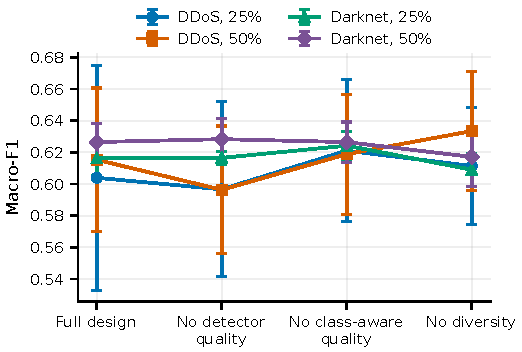
\includegraphics[width=0.96\columnwidth]{figures/eval_component_ablation.pdf}
    \caption{Paired Macro-F1 change after removing one secondary component.
    Points distinguish the 25\% and 50\% budgets; horizontal bars are 95\%
    confidence intervals over five protocol seeds.}
    \label{fig:eval-component-ablation}
\end{figure}

\bheading{Semantic parameters} On two fixed DARKNET partitions and two
architectures, varying $n_{\min}\in\{1,2,5,10\}$ and replacing
inverse-square-root class weights with uniform weights leaves the selected
set, semantic coverage, Macro-F1, and worst recall unchanged across the tested
grid.

\bheading{Learner architecture} We evaluate all four combinations of
XGBoost~\cite{xgboost} and LightGBM local/global
learners.  L+X is best on DDOS, L+L is best on MALDROID and DARKNET, and X+L
and L+L tie on DOH.  The pipeline supports both learner families, with the
strongest backend sensitivity appearing on DDOS.

\begin{table}[t]
    \centering
    \caption{\Fname accuracy for four local/global learner combinations.
    X and L denote XGBoost and LightGBM, respectively; values are means over
    five protocol seeds.}
    \label{tab:eval-architecture}
    \footnotesize
    \setlength{\tabcolsep}{3.8pt}
    \begin{tabular}{@{}lrrrr@{}}
        \toprule
        Dataset & X+X & L+X & X+L & L+L \\
        \midrule
        DDOS     & 0.621 & \textbf{0.642} & 0.641 & 0.624 \\
        MALDROID & 0.826 & 0.854 & 0.847 & \textbf{0.860} \\
        DARKNET  & 0.824 & 0.826 & 0.829 & \textbf{0.832} \\
        DOH      & 0.801 & 0.800 & \textbf{0.807} & \textbf{0.807} \\
        \bottomrule
    \end{tabular}
\end{table}

\bheading{Answer to RQ3} The selected solution is invariant across the tested
semantic-parameter grid, and the pipeline supports all four learner
combinations.  Component and backend choices provide dataset-specific tuning
opportunities.

\subsection{RQ4: What Utility Remains after Laplace Perturbation?}

We can perturb every selected score block before logical upload.  To isolate
utility sensitivity, we freeze the 50\%-budget selection first and
then add independent Laplace noise with scale $2/\epsilon$ to stacker-fit
encodings.  We compare this selected configuration with all 66 encoders on
DDOS over five protocol seeds, keeping test encodings fixed for evaluation.
This centralized replay samples the distribution in
Eq.~\ref{eq:local_laplace_release}; the execution model of
Theorem~\ref{thm:local_score_privacy} instead draws fresh private randomness at
each client before upload.

Table~\ref{tab:eval-laplace} reports Macro-F1 for no noise and
$\epsilon\in\{50,20,10,7,5,3,1\}$.  Here, $\epsilon$ controls the per-block
perturbation and the corresponding noise scale is $2/\epsilon$.  At the
strongest tested perturbation ($\epsilon=1$), Macro-F1 falls from 0.6153 to
0.5105 for the
50\%-budget selection and from 0.6412 to 0.5298 for all encoders.  The
intermediate means fluctuate as $\epsilon$ decreases; the largest observed
drop occurs at $\epsilon=1$.

\begin{table}[t]
    \centering
    \caption{Macro-F1 sensitivity to per-block Laplace perturbation on DDOS.
    Five-seed means are reported with 95\% confidence intervals.}
    \label{tab:eval-laplace}
    \footnotesize
    \setlength{\tabcolsep}{3.0pt}
    \begin{tabular}{@{}lrrr@{}}
        \toprule
        $\epsilon$ & Noise scale & Selected (50\%) & All 66 \\
        \midrule
        No noise & 0     & $0.6153\pm0.0453$ & $0.6412\pm0.0121$ \\
        50       & 0.04  & $0.5861\pm0.0439$ & $0.6037\pm0.0078$ \\
        20       & 0.10  & $0.5932\pm0.0244$ & $0.5999\pm0.0234$ \\
        10       & 0.20  & $0.5910\pm0.0117$ & $0.5918\pm0.0191$ \\
        7        & 0.286 & $0.5939\pm0.0136$ & $0.5874\pm0.0174$ \\
        5        & 0.40  & $0.5875\pm0.0091$ & $0.5777\pm0.0163$ \\
        3        & 0.667 & $0.5655\pm0.0120$ & $0.5870\pm0.0046$ \\
        1        & 2.00  & $0.5105\pm0.0301$ & $0.5298\pm0.0400$ \\
        \bottomrule
    \end{tabular}
\end{table}

\bheading{Answer to RQ4} The seven perturbation levels expose a
utility--perturbation profile: intermediate means fluctuate, while
$\epsilon=1$ produces the largest observed utility drop.  Together with
Theorem~\ref{thm:local_score_privacy}, these results connect the Laplace
release rule to its measured stacker utility.
% TODO(author): The replay does not instantiate a client-side trust boundary.
% End-to-end privacy additionally requires release composition, and the stated
% theorem does not cover labels or the remaining protocol messages.

\subsection{RQ5: Is the Selector and Pipeline Practical?}

\bheading{Exactness and scaling} We first compare the bitmask dynamic program
with exhaustive lexicographic search on a suite of small oracle instances.
The primary coverage value agrees throughout the suite, and repeated runs are
deterministic.  Figure~\ref{fig:eval-solver-scaling} then separates growth in
the number of semantic classes $C$ from growth in the candidate count $M$.
At the main-scale point $M=66,C=12$, the isolated solver uses a median of
1.99 seconds, reaches 2,829 states, and peaks at 98.27 MiB RSS.  Increasing
$M$ to 256 at $C=12$ raises median time to 33.73 seconds, whereas increasing
$C$ to 20 at $M=66$ reaches 460,405 states, 100.10 seconds, and 580.45 MiB.
Thus, semantic dimension, rather than candidate count alone, is the dominant
capacity driver.

\begin{figure}[t]
    \centering
    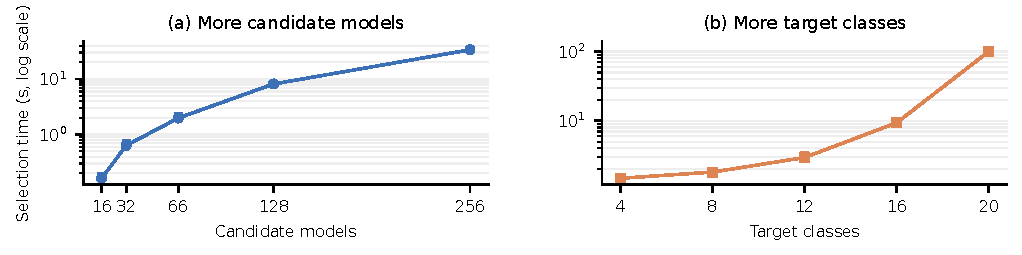
\includegraphics[width=0.96\columnwidth]{figures/eval_solver_scaling.pdf}
    \caption{Sparse dynamic-program scaling.  The blue and rose trajectories
    independently vary semantic classes and candidates using separate fixed
    fixtures.  Both axes are logarithmic; whiskers extend from median to
    95th-percentile time over ten repeats.}
    \label{fig:eval-solver-scaling}
\end{figure}

\bheading{End-to-end replay cost} Table~\ref{tab:eval-system-cost} integrates
wall-clock and logical-communication evidence.  Full
group time includes all reported methods and repetitions, whereas the
preceding microbenchmark isolates one primary solve.  Stacker fitting is the
largest measured stage on MALDROID, DARKNET, and DOH; the multi-method
selection stage is largest on DDOS.  At the 50\% budget, \Fname reduces total
logical payload by approximately half on each dataset.

\begin{table*}[t]
    \centering
    \caption{Single-machine replay time and logical payload.  Times are means
    over five protocol seeds.  ``Dominant'' is the largest recorded stage;
    logical reduction compares \Fname with all encoders.}
    \label{tab:eval-system-cost}
    \footnotesize
    \setlength{\tabcolsep}{3.2pt}
    \begin{tabular}{@{}lrlrrrr@{}}
        \toprule
        Dataset & Total group (s) & Dominant stage & Stage time (s) & All (MiB) & \Fname (MiB) & Reduction \\
        \midrule
        DDOS     & 3,005.16 & Selection     & 1,026.34 & 7,040.05 & 3,489.07 & 50.4\% \\
        MALDROID & 47.03    & Stacker fit   & 35.21    & 662.66   & 335.94   & 49.3\% \\
        DARKNET  & 2,550.50 & Stacker fit   & 2,272.66 & 3,436.78 & 1,732.29 & 49.6\% \\
        DOH      & 512.34   & Stacker fit   & 170.04   & 2,942.76 & 1,488.51 & 49.4\% \\
        \bottomrule
    \end{tabular}
\end{table*}

\bheading{Answer to RQ5} The solver exactly matches exhaustive search
throughout the oracle suite and completes the 66-candidate benchmark in
1.99 seconds.  Scaling isolates semantic dimension as the dominant capacity
driver, while the end-to-end replay confirms an approximately 50\% reduction
in logical payload.
% TODO(author): Exactness is conditioned on completing below the configured
% state cap; physical network latency is outside the current replay.

\endgroup
